\documentclass[a4paper, 12pt]{report}
\usepackage[a4paper, top=2cm , bottom=2cm , right=2cm , left=2cm ]{geometry}

\usepackage{graphicx} % Required for inserting images
\usepackage[T1]{fontenc}
\usepackage[english]{babel}
\usepackage[utf8]{inputenc}
\usepackage{titlesec}
\usepackage{xcolor}
\usepackage{amsfonts}
\usepackage{wrapfig}
\usepackage{amssymb}
\usepackage{amsbsy}
\usepackage{float}
\usepackage{soul}
\usepackage[makeroom]{cancel}
\usepackage[framemethod=tikz]{mdframed}
\usepackage{mathtools}
\usepackage{matlab-prettifier}
\usepackage{subcaption}
\usepackage{bm}
\usepackage{tikz}
\usepackage{colortbl} % for cell color in matrices
\usepackage{booktabs}
\usepackage{amsmath}
\usepackage{xcolor}
\usepackage{tcolorbox}
\usepackage{tikz} %for block diagrams
\usepackage{amssymb}
\usepackage{enumitem} 
\usetikzlibrary{positioning}
\usepackage{xcolor}

\definecolor{myblue}{RGB}{30, 131, 197}
\definecolor{mygreen}{HTML}{25da18}
\definecolor{myyellow}{RGB}{255, 255, 0}
\definecolor{mygrey}{RGB}{100, 100, 100}
\definecolor{myred}{RGB}{255, 55, 55}

\newtcolorbox{factbox}[1][]{
    colback=mygreen!5,   % Background color
    colframe=mygreen!30, % Frame color
    fonttitle=\bfseries,  % Title font
    title=#1,             % Title
    coltitle = black,   %title color
    sharp corners=southwest,
}
\newtcolorbox{QandAbox}[1][]{
    colback=myred!5,   % Background color
    colframe=myred!20, % Frame color
    fonttitle=\bfseries,  % Title font
    title=#1,             % Title
    coltitle = black,   %title color
    sharp corners=southwest,
}

\newtcolorbox{example}[1][]{
    colback=mygrey!3,   % Background color
    colframe=mygrey!20, % Frame color
    fonttitle=\bfseries,  % Title font
    title=#1,             % Title
    coltitle = black,   %title color
    sharp corners=southwest,
}
% Do not indent paragraphs
\usepackage[parfill]{parskip}

\lstset{
    basicstyle=\ttfamily\scriptsize,
    keywordstyle=\color{blue},
    commentstyle=\color{green!60!black},
    stringstyle=\color{red},
    numbers=left,
    numberstyle=\tiny,
    stepnumber=1,
    numbersep=8pt,
    frame=single,
    breaklines=true,
    captionpos=b
}


% In case of an image at the bottom, but the footnote below the image (without this the image will be below the footnote)
\usepackage[bottom]{footmisc}

% --------- CUSTOM HEADER ----------
\input{customizations/header.tex}

% ------------ NEW ENVS ------------
\input{customizations/environment.tex}

% ---------- NEW COMMANDS ----------
\input{customizations/commands.tex}


% Make references clickable and change style of links to blue
\usepackage{hyperref}
\hypersetup{
	colorlinks=true,
	linkcolor=blue,
	filecolor=magenta,      
	urlcolor=cyan,
}

\graphicspath{ {images/} }

\input{customizations/title-spacing.tex}

\title{
    \textbf{\Huge{Laboratory of Robust Identification and Control}}\\
    \textit{Lecture notes}
}
\author{A. Ayanmanesh Motlaghmofrad}
\date{A.Y. 2024/2025}


% Force all math to use \displaystyle by default
\everymath{\displaystyle}

\linespread{1.2} % Adjusts line spacing to 1.5

\begin{document}
\maketitle
\tableofcontents


% ---------------------------------------------------------------------
% ------------------------ MODIFY ONLY BELOW --------------------------
% ---------------------------------------------------------------------
% ---------------------------------------------------------------------

\chapter{Introduction}    % For a new chapter (works in book and report class)
\subsubsection{Disturbances and uncertainties}
% page1
% -------------------------------------

    The key word \textit{Robust} suggests that we are taking uncertainties into account. The model of the plant is as following:

%Graph
\begin{figure}[htbp]
    \centering
    \includegraphics[width=\textwidth]{images/1.png} % Adjust width as needed
    \caption{A general control plant with additive disturbances \textit{l} and \textit{d}}
    \label{fig:graph_label}
\end{figure}


The general nonlinear state-space representation of the system is:

\begin{equation}
    \begin{cases}
    \dot{x}(t) = f(x(t), u(t)) \\
    y(t) = g(x(t), u(t))
    \end{cases}
\end{equation}
Where:
\begin{itemize}
    \item $x(t)$ is the state vector,
    \item $u(t)$ is the input vector,
    \item $y(t)$ is the output vector,
    \item $f(\cdot)$ is a nonlinear function describing the system dynamics,
    \item $g(\cdot)$ is a nonlinear function describing the output equation.\\
\end{itemize}

%page 2
%--------------------------------------------------
    \textbf{The first step} of any control problem is typically \textbf{derivation of mathematical model of the plant.} This step is the most crucial step, because if we drive the model by applying first principles of physics, we are likely to adopt approximated models, adopting simplifying assumptions, e.g. rigid body assumption etc. Further, the value of the physical parameters involved in the equations, such as friction coefficient, are not exactly known. Such approximations introduce errors and uncertainty in the mathematical description of the plant to be studied and controlled.

% page 3
% -----------------------------------------------------
    This fact is critical, since standard approaches to controller design are model-based; that is, the controller design has a strong dependency on the mathematical models used to describe the plant to be studied and controlled.


\begin{center}
$\textit{\textbf{Neglecting some physical details}} \equiv \textit{\textbf{Neglecting some state variables}}$
\end{center}

    For example, for modelling a robotic arm, generally, rigidity is assumed for the joints. Nevertheless, in fast movements  this assumption does not hold anymore, and the model does not predict the real performance of the robot, neglecting some state variables. Further, in some applications, we are not even aware of the phenomenon or phenomena that is being neglected. 

\subsubsection{Counter act for disturbances and uncertainties}

\begin{itemize}
    \item \textbf{First counter act}  These uncertainties and disturbances directly affect the controller design in the time domain, since the feedback gain and observer are directly calculated by solving algebraic equations including physical parameters with uncertainties. Nontheless, In frequency domain, the design of the controller is less affected by these uncertainties. 

    This does not mean that \textit{Transfer Function} is not affected by uncertainties of the parameters, because not considering some phenomona leads to the transfer function having less poles or zeros and because the uncertainty of the parameters affect the coefficients of the complex variables, being \textit{s} or \textit{z}. In the frequency domain design, we design the controller based on the frequency response of the system, considering cutting frequencies that reject high-frequency and low-frequency disturbances. In addition, by considering phase-margin and gain-margin, some margin for disturbances and uncertainties are taken into accoutn.

\textbf{Question to be answered: the sensitivity function is high-pass filter, meaning that the high frequency phenomenon, on the other-hand T is a low-pass filter, if the plant is designed for having a fast rising time, high-frequency phenomena also passes T.}

    \item \textbf{Second counter act}: Optimization problems in state-space where introduced to tackle this problem.
    \item \textbf{Third counter act}: Optimization problem, in state space, is combined with the concept of robustness, in frequency space, which is called $H_{\infty}$. 
\end{itemize}


\subsubsection{What is going to be discussed in this course}
    In the first part of this course, we are going to learn how to learn from the mapping from the input to the output of the system, extracting a \textbf{mathematical model} for the plant. Further, it elaborates on this data to drive also a \textbf{discription for uncertainty}. These, together, can be used for \textbf{robust controller design} in a model-based approach.

    In the second step, the aim is to design a controller directly from the data, without the intervention of the model.


\begin{factbox}[Professor's Quote]

    In conclusion, even if the physical model is very precise, at some point, in order to measure the parameters used in the physical models, it is required to do some experimental measurements, subjected to noise, introducing uncertainties to our model.\newline \newline
    If these uncertainties are not taken into account, the controller will not have a good performance when implemented physically, and it is going to work only in simulations. \newline \newline
    There are many approaches to tackle this problem. Here, in the first part of the course, we will focus on \textbf{System Identification}, which is another modelling paradigm. In this paradigm, we learn the mathematical model of the system to be controlled by using experimentally collected data. Not only do we introduce what \textit{System identification} is and what are the possible approached, but maintly to focus on \textbf{\textit{Set-membership Identification Technique}} that allow us to learn the model of the system, and drive information about how the uncertainty is affecting out model; this is used to design a controller in a robust manner. Robust controller designed can be directly applied to the real physical plants.  \newline \newline
    
    In the second part of the course, we shift our paradigm again. In this part, assuming that the collected data represents the behavior of the mapping between the input and output, we try to design the controller directly from the data, called  \textbf{Direct Data-Driver Controller Design}. \newline \newline
    
\end{factbox}


\chapter{System Identification}    % For a new chapter (works in book and report class)
\subsubsection{What system identificaiton is about?}
% page7
% -------------------------------------
\textit{System identification} deals with the problem of building mathematical model of dynamical systems from sets of experimentally collected input, output data.


\begin{figure}[htbp]
    \centering
    \includegraphics[width=0.5\textwidth]{images/system-id-scheme.png}
    % Adjust width as needed
    \caption{Classifications of System Identification Problems}
    \label{fig:id_classes}
\end{figure}

There are three different approaches to mathematically model dynamical systems:
\begin{enumerate}

\item \textbf{White-box modelling}:\newline Models, in this approach, are obtained by applying \textbf{first principles for physics}. All the physical phenomena and also all the physical parameters involved in the equiation are assumed to be exactly know. This approach was applied in the course of \textit{Automatic Control} for modelling systems.

\item \textbf{Grey-box modelling}: Here, \textbf{models} are base on the equations obtained by applying first principles of \textbf{physics}, but \textbf{the parameters} entering the equations are not completely known, so they need \textbf{to be estimated} from experimental data. 

\item \textbf{Black-box modelling}: In this case, the structure of the equations is selected by the user on the basis of some \textbf{"general" a-priori information}, e.g. linearity, on the system physics, or at any rate by the system properties. \newline 

\begin{factbox}[Professor's Quote]
    In this method, the designer of the system model, has some degree of freedom in selecteing the structure of the model, provided that the model embeds the "general" a-priori information.\newline \newline
    If we do not have any a-priori information, an artificial-neural-network may be selected as the structure of the model.
\end{factbox}
the parameters involved in the equations of the black-box models are \textbf{to be estimated}, or computed, by using experimentally collected data. In general, \textbf{the parameters of a black-box model do not have a clear physical meaning}.
\end{enumerate}


In general, \textbf{white-box models are not very useful in practice}, at least for control applications, because they are based on the assumption that the physics involved in the system under study is well-known.

\subsubsection{The comparison between the grey-box and Black-box models:}
\textbf{Similarity} 
In both cases:
\begin{itemize}
\item physical insight is exploited to drive/select the structure of the equations.
\item experimentally collected data is used to estimate/compute the parameters involved in the equations.
\end{itemize}

\textbf{Difference} 
\begin{itemize}
\item In grey-box modelling, the structure of the equations is not selected by the user, since it is forced by the first principles of physics. This suggests that, in general, the equations of a grey-box model depends, in a possibly complex, non-linear ways, on the physical parameters to-be-estimated.\newline
for instance of a grey-box model:
$\begin{cases}
    \dot{x}(t) = A x(t) + B u(t) \\
    y(t) = C x(t) + D u(t)
\end{cases}$ where:
\newline
\[
A = \begin{bmatrix}
\frac{m}{k^2} & \sqrt{\beta} \\
\frac{\alpha^2.k^3}{\gamma} & 1  
\end{bmatrix}, \quad
B = \begin{bmatrix}
b_1 \\
b_2
\end{bmatrix}, \quad
C = \begin{bmatrix}
c_1 & c_2
\end{bmatrix}, \quad
D = \begin{bmatrix}
d
\end{bmatrix}
\]
In this case, using the physical principles for modelling seems like a good idea; the system is simple, and its physics is well-known. The problem is that the parameters are to-be-estimated. This problem leads to an optimization problem. Now, A difficulty may arise, because if the equation we are going to write so that they relates input and output data obtained experimentally depends on parameters in a complex and non-linear fashion, the mathematical problem of driving what are the correct value of the system parameter satisfying the relation between the intput and output is going to be a complex problem. \textbf{This is the main limitation of grey-box model.}

\item In the black-box version of the same problem, just some general information such as liniearity and time-invariantion is exploited. Now, we found the four matricies \textit{A, B, C, D} in a form that is much simpller, just 4 parameters for A, and so on, for instance. In this case, the system output depends on the input in a way simpler manner.
\[
A = \begin{bmatrix}
a_{11} & a_{12} \\
a_{21} & a_{22}  
\end{bmatrix}, \quad
B = \begin{bmatrix} 
b_1 \\
b_2
\end{bmatrix}, \quad
C = \begin{bmatrix}
c_1 & c_2
\end{bmatrix}, \quad
D = \begin{bmatrix}
d
\end{bmatrix}
\]\newline


\begin{factbox}[Professor's Quote]
    Therefore, in black-box model, we have more freedom to select the struture of the equations in a way that is computationally more convenient, by embedding/exploiting some general properties drived from our physical insight. 
The idea is to consider only the most important a-priori information and/or the information that we trust the most!
\end{factbox}

\end{itemize}

\subsubsection{General procedure for building a grey/black-box modelling:}
Let's compare grey-box and black-box models from the point of view of the parameter estimation problem. While building the mathematical model of the system, in general, we follow a procedure similar to the following one, it be a grey-box or black-box structure:\newline

\begin{enumerate}
    \item to exploint availabe a-priori information on the system under study to select \textbf{the structure of the mathematical equation} describing the input-output mapping.
    \begin{factbox}[Professor's Quote]
The model is always in the input/output form. Signals that we can apply to the system is called input, and signals that we can measure, is called output. If we are in the case where we can measure all \textbf{state variables} involved in the system, we can have a full description of the system. However, in a general case, the system involves input, output, and state variables, but we are able to measure only a subset of physical variables in the system - being the value to be monitored or the control output.

Now, these parameters have physical meaning in grey-box case, or are merely mathematical parameters in black-bock case.
\end{factbox}

In the end of this step, we have a mathematical model of the following form:
\begin{equation}
y(t) = f\left( u(t), \theta\right)
\end{equation}

    \item To collect input-output data representing the behavior of the system under study by performing an experiment. $\tilde{u}$ and $\tilde{y}$ are noise-corrupted data, since, in general, noise can corrupt the output measurements as well as measurement of the input signal applied to the system.
\begin{center}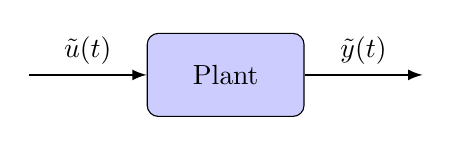
\begin{tikzpicture}[auto, node distance=2.5cm, >=latex]
    % Define styles
    \tikzstyle{block} = [rectangle, draw, fill=blue!20, 
                          text width=5em, text centered, rounded corners, minimum height=3em]
    \tikzstyle{input} = [coordinate]
    \tikzstyle{output} = [coordinate]
    \tikzstyle{arrow} = [thick,->,>=latex]
    
    % Nodes
    \node [input] (input) {};
    \node [block, right of=input] (plant) {Plant};
    \node [output, right of=plant] (output) {};
    
    % Draw arrows
    \draw [arrow] (input) -- node [above] {$\tilde{u}(t)$} (plant);
    \draw [arrow] (plant) -- node [above] {$\tilde{y}(t)$} (output);
\end{tikzpicture}\end{center}
    \item To formulate a suitable mathematical problem to estimate/compute the values of the vector of parameters $\theta$ in such a way that our mathematical model is going to describe the behavior of real system as well as possible.
for example:
\[
\hat{\theta} = \arg \min\limits_{\theta \in S} f(\theta) = \arg \min\limits_{\theta} \|\tilde{y} - f(\tilde{u}, \theta)\|_2
\] 
J(.) here is a \textbf{cost function}. In this case, it is the euclidian norm of $\tilde{y}$ and $f(\tilde{u}, \theta)$.\\
\end{enumerate}
\newpage
At the third stage, the difference between grey-box and black-box models comes into play, since:
\begin{itemize}
    \item In grey-box model: $f(\tilde{u},\theta)$ will, in general depends in a complex, non-linear manner from $\theta$, \textbf{leading to multi-minima convex cost function which is really hard to be minimize}\\ \\
    While\\
    \item In black-box model: $f(\tilde{u},\theta)$ will be selected by the user in order to depend linearly from $\theta$,if possible, or in the simplest possible way, \textbf{leading to a single-minima convex funciton to be minimized}, which is much easier in comparison. \\
\end{itemize}
For example, consider the following multi-minima cost-function: \\

\(
J(\theta_1, \theta_2) = \sin(\theta_1) \cdot \cos(\theta_2) + \frac{\theta_1^2 + \theta_2^2}{10}
\)

\begin{figure}[htbp]
    \centering
    \includegraphics[width=0.75\textwidth]{images/multi-minima-cost-function.png}
    % Adjust width as needed
    \caption{The 3D plot and countor plot of the afforementioned cost-function, which is a multi-minima cost-function}
    \label{fig:multi-minima-cost-function}
\end{figure}

In this example, we look for the global minimum of the cost-function. Finding this point, however, is not an easy task, due to the fact that there is no guarantee that our optimization algorithm will not be trapped in one of the local minima, which may correspond to a "very bad" estimation of $\theta$. Even if we find the global minimum by chance, there is no guarantee that output is indeed the global minima.

On the other hand, When a black-box model is considered, a parametrization is considered so that the function $f(u,\theta)$ is a convex function of $\theta$, thereby having a single global minimum. In this case, no matter what optimization algorithm is used, reaching the global minimum is guaranteed.This is evident in the following cost-function:\\

\(
J(\theta_1, \theta_2) = \theta_1^2 + \theta_2^2
\)
    
\begin{figure}[htbp]
    \centering
    \includegraphics[width=0.75\textwidth]{images/convex-cost-function.png}
    % Adjust width as needed
    \caption{The 3D plot and countor plot of the afforementioned cost-function, which is a convex cost-function}
    \label{fig:multi-minima-cost-function}
\end{figure}


\begin{QandAbox}[Q and A]
    \textbf{Question:} we use grey-box model when we have an insight about the system and parameters. Hence, when we run the optimization problem, we can initialize the optimization problem with more suitable initial condition. Further, we can neglect some of the estimation, knowing that the estimated value does not correspond to the physical quantity the parameter is expected to have.\\
    
    \textbf{Professor's answer:} This is true for simple systems. Nonetheless, in such compolex systems as chemical processes or optical lazer systems, it's hard to have an insight before hand about some parameters. In addition, since we are dealling with multi-dimensional problems, it might be the case that we confine the expected value for some parameters but still, for some parameters, we need to deal with the issue mentioned about the multi-minima cost functions. However, it might be the case that the estimation of those physical parameters are of interest, which is not the concern of this course. Here, we do system identification for control purposees. \\
    
\end{QandAbox}

To clarify the matter further, consider an \textbf{\textit{LTI system}} such that the \textbf{transfer function} obtained from \(H(s) = C (sI - A)^{-1}B +D\) where matrices \(A, B, C, D\) are teh state-space matrices obtained by applying the first principles of physics.\\

\(
H(s) = \frac{ \frac{P_1²}{P_2} s + \frac{P_3}{\sqrt{P_4}}}{s^2 + \frac{P_1.P_2}{P_3^3} + 1}
\)\\

Where \(P_1, P_2, P_3, P_4\) are the physical parameters. Now, in terms of modelling the input-output behavior of the system, we don't miss anything by considering the following transfer function.\\

\(
H(s) = \frac{\theta_1 s + \theta_2}{s^2 + \theta_3 s + \theta_4}
\)\\

In this black-box model, we just take into consideration the most important "general" information that the system is an LTI system - hence being able to be modelled as a transfer function - and of order two. Therefore, we can use a transfer function model for describing the system behavior.\\

\begin{factbox}["Phylosophical Remark"]
    Pay attention that \textbf{we cannot build our model without any assumption about the system}. No matter how much input-output sample is available,  we need to have an assuption about the system to be able to descibe it.
\end{factbox}

In conclusion: \\
\textbf{black-box models} are thet best choice for the following purposes:
\begin{itemize}
    \item simulalting the input-output behavior of the system
    \item modelling for the purpose of designing a controller\\
\end{itemize}

\textbf{Grey-box models}, in general, are the best choice when it is desired to:
\begin{itemize}
    \item estimate the values of some physical parameters \\
\end{itemize}

If the physical systeme is well-known, \textbf{white-box modelling} is the choice.


\chapter{Set-membership identification}    % For a new chapter (works in book and report class)

Set-membership approach is an alternative to the classical, statistical identification approach. Least-Square method is one possible example of statistical estimation algorithms in the context of estimation.\\

\subsubsection{Main ingredients}

We consider a discrete-time system described in the following parametrized regression form:\\
\begin{equation}
y(k) = f(y(k-1), y(k-2), \cdots, y(k-n), u(k), u(k-1), \cdots, u(k-m), \theta_1, \theta_2, \cdots, \theta_{n+m+1})
\end{equation}

where \(m\leq n\)\\
A-priori information on the system:
\begin{itemize}
    \item \(n\) and \(m\) are known
    \item \(f \in \mathbb{F}\) where \(\mathbb{F}\) is the class of model selected on the basis of our physical insight. 
\end{itemize}


A-priori information on the noise, the main difference with respect to the previous discussion.
\begin{itemize}
    \item the noise structure is known, i.e. the way the way uncertainty affects the input-output data)
    \item the noise is assumed to belong to konwn bounded set \(\mathbb{B}\).
\end{itemize}

When the consistency property of LS was discussed, and in general statistical approach to system identification, the typicall assumption on the noise is that statistical distribution of the noise sequence, or the value of some moments of inertia of the noise is known, such as variance. Here, the assumption is that the noise sequence \(\eta\) belongs to a bounded \(\mathbb{B}\). Remember that assumption two of the consistency property was the crucial one, so a change of perspective is adopted on the second assumption, where we deal with the following problem:

\textbf{Set-membership identification of LTI system} under the assumption that the uncertainty affecting the data can be modelled as an equation error \(e(k)\), which is exactly assumption \(1\) considered for the consistency theorem.\\
\[
\begin{aligned}
\tilde{y}(k) = & -\theta_1 \tilde{y}(k - 1) - \theta_2 \tilde{y}(k - 2) - \cdots - \tilde{y}(k - n) \\[1ex]
               & + \theta_{n+1} \tilde{u}(k) + \theta_{n+2} \tilde{u}(k - 1) + \cdots + \theta_{n+m+1} \tilde{u}(k - m) + \mathbf{e(k)} \\[2ex]
\end{aligned}
\]
where,
\[
\begin{aligned}
e(k) \in \mathbb{B}e = \left\{ \bar{e} = [e(1), e(2), \cdots, e(H)]^T \right\} : \left| e(k) \right| \leq \Delta e, \forall k
\end{aligned}
\]
where  \(\Delta e \) is a given real bounded constant.

\begin{factbox}[]
In set-membership, we always have unknown and bounded assumption about the magnitude of noise.\\

The bound is considered a conservative bound.

\end{factbox}
\subsubsection{Error-in-Variable setting}
Let's assume that the data are actually collected from a real experiment, which is EIV setup. The block-diagram representation of this a-priori information is as follows.

\begin{center}
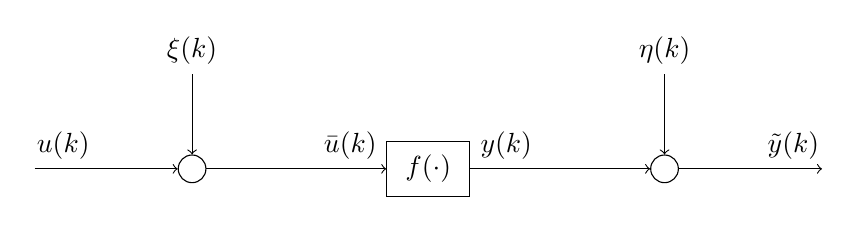
\begin{tikzpicture}[auto, node distance=2cm]

    % Block styles
    \tikzstyle{block} = [draw, rectangle, minimum height=2em, minimum width=3em]
    \tikzstyle{sum} = [draw, circle, inner sep=0pt, minimum size=1em]
    \tikzstyle{input} = [coordinate]
    \tikzstyle{output} = [coordinate]

    % Nodes
    \node [input] (input) {};
    \node [sum, right of=input, node distance=2cm] (sum1) {};
    \node [block, right of=sum1, node distance=3cm] (system) {$f(\cdot)$};
    \node [sum, right of=system, node distance=3cm] (sum2) {};
    \node [output, right of=sum2, node distance=2cm] (output) {};

    % Connections
    \draw [->] (input) -- node[pos=0.2] {$u(k)$} (sum1);
    \draw [->] (sum1) -- node[pos=0.8] {$\bar{u}(k)$} (system);
    \draw [->] (system) -- node[pos=0.2] {$y(k)$} (sum2);
    \draw [->] (sum2) -- node[pos=0.8] {$\tilde{y}(k)$} (output);
    
    % Noise terms
    \node [above of=sum1, node distance=1.5cm] (xi) {$\xi(k)$};
    \draw [->] (xi) -- (sum1);
    
    \node [above of=sum2, node distance=1.5cm] (eta) {$\eta(k)$};
    \draw [->] (eta) -- (sum2);

\end{tikzpicture}
\end{center}

\textit{Errors-in-variables} (EIV) problems refer to the most general case where both the input and the output collected samples are affected by noise.

\[
\xi = [\xi(1), \dots, \xi(H)] \in \mathcal{B}_{\xi}
\]
\[
\eta = [\eta(1), \dots, \eta(H)] \in \mathcal{B}_{\eta}
\]

$\mathcal{B}_{\xi}$ and $\mathcal{B}_{\eta}$ are bounded sets described by \textbf{\textit{polynomial constraints}.}

Most common case:
\[
\mathcal{B}_{\eta} = \left\{\eta : |\eta(k)| \leq \Delta_{\eta}\right\}, \quad \mathcal{B}_{\xi} = \left\{\xi : |\xi(k)| \leq \Delta_{\xi}\right\}
\]
Here, $f(.)$ belogn to a class of function $\mathbb{F}$, which is the a-priori assumption on the system.\\

Considering this a-priori information about the structure of the course, and a-priori information about the system, which is LTI second-order system. The noises can be reformulated as \textbf{Error-in-Equation}, which is the same as the first assumption of the consistency property of Least Square.


\[
\begin{array}{l}
\tilde{y}(k)= -\theta_1 \tilde{y}(k - 1) - \theta_2 \tilde{y}(k - 2) + \theta_3 \tilde{u}(k) + \theta_4 \tilde{u}(k - 1) + \theta_5 \tilde{u}(k - 2) \\[1ex]
\textcolor{red}{\fbox{\textcolor{black}{$+ \theta_1\eta(k-1) + \theta_2\eta(k-2) - \theta_3\tilde{u}(k) - \theta_4\tilde{u}(k-1) - \theta_5\tilde{u}(k-2) + \eta(k) $}}} =: + e(k) \\
\end{array}
\]

Up till now, nothing is changes, we now that statistically this kind of error is not i.i.d. The difference in is regarding the second assumption about the noise, \(e(k)\), which is the boundedness of the noise:

\[\left| e(k)\right| \leq \Delta e \forall k = 1, 2, ..., N\]

Provided that we find a way to compute the bound \(\Delta e \), on \(\left| e(k)\right|\), the identification problem can be correctly formulated in terms of \textbf{Equation-Error} structure in Set-membership framework. \textbf{However, Computing \(\Delta e \) is not an easy task}. Since it cannot be done without any assumption about \(\theta_i\), since they are to be identified.

\subsubsection{Set-membership formulation of the problem identifying a second order LTI system assuming an Equation-Error structure for the uncertainty}
Main ingredients:
\begin{enumerate}
\item \textbf{a-priori information }about the system, second order LTI, and the noise, Equation-Error structure and boundedness.
\item\textbf{ a-posteriori information} are experimentally collected input-output data samples.
\end{enumerate}
Now, here, we have the concept of \textit{Feasability Parameter Set}.

\subsubsection{Feasability parameter set}
The feasability parameter set \(\mathbb{D}_\theta\) is the set of all the values of the parameter vector \(\theta = \left[ \theta_1 \theta_2 \cdots \theta_p \right]^T \in \mathbb{R}^p\), which are consistent with all the avialable information on the system and the noise, and all he collected data.\\
To better understand the meaning of FPS, \(\mathbb{D}_\theta\), let's assume that we are collecting data according to the following\textbf{ Output-Error} setup:\\

\begin{center}    % Block styles
\begin{tikzpicture}[auto, node distance=2cm]

    \tikzstyle{block} = [draw, rectangle, minimum height=2em, minimum width=3em]
    \tikzstyle{sum} = [draw, circle, inner sep=0pt, minimum size=1em]
    \tikzstyle{input} = [coordinate]
    \tikzstyle{output} = [coordinate]

    % Nodes
    \node [input] (input) {};
    \node [block, right of=input, node distance=3cm] (system) {$f(\cdot)$};
    \node [sum, right of=system, node distance=3cm] (sum2) {};
    \node [output, right of=sum2, node distance=2cm] (output) {};

    % Connections
    \draw [->] (input) -- node[pos=0.5] {$u(k)$} (system);
    \draw [->] (system) -- node[pos=0.2] {$y(k)$} (sum2);
    \draw [->] (sum2) -- node[pos=0.8] {$\tilde{y}(k)$} (output);
    
    % Noise terms at the output
    \node [above of=sum2, node distance=1.5cm] (eta) {$\eta(k)$};
    \draw [->] (eta) -- (sum2);
\end{tikzpicture}
\end{center}\vspace{1cm}


Since, we have the following form of noise:\\
\[y(k) = \tilde{y} - \eta(k)\]
and we know that \(\eta\) is bounded. we can obtain the following relationship about the \(y(k)\), being that the real \(y(.)\) signal is enveloped in the following fashion:\\
\[
\tilde{y}(k) - \eta{k} \leq y(k) \leq \tilde{y}(k) + \eta{k}
\]

\begin{figure}[htbp]  % "h" for here, "t" for top, "b" for bottom, "p" for float page
    \centering
    \includegraphics[width=0.75\textwidth]{images/FPS_time_domain.jpg}
    \caption{The bounds for \(y\) encompass all the elements of the \(\theta\) vector, leading to a relation for \(y\) such that its graph is bounded between the represented bounds.}
    \label{fig:FPS_time_domain}
\end{figure}

\begin{factbox}[Professor's Quotes]
In the statistical identification, assuming probabilistic characteristics for the noise, instead of having bounded interval around each single sample of the output that we collect, we have a normal distribution around each single point. Therefore, a correct formulation of the identification, again, in that context, lead to a set of models, but this time instead of having a bounded set of possible models solving the problem, we obtain a set that is statistically described, where each models have a certain probability of being the correct model.
\end{factbox}

Now, let's try to define mathematically, the FPS \(\mathbb{D}_\theta\)
\[
\begin{aligned}
\mathbb{D}_\theta = \{
\theta = \left[\theta_1 \, \theta_2 \, \cdots \, \theta_p \right]^T \in \mathbb{R}^p \, | \, 
\tilde{y}(k) = & -\theta_1 \tilde{y}(k - 1) - \theta_2 \tilde{y}(k - 2) + \theta_3 \tilde{u}(k) + \theta_4 \tilde{u}(k - 1) \\
& + \theta_5 \tilde{u}(k - 2) + e(k) \, | \, \forall k > 3 \,,\, |e(k)|\leq \Delta e
\}
\end{aligned}
\]
However, this mathematical description is not correct, since here we define FPS as a subset of \textbf{parameter space}, \(\mathbb{R}^p\), but the description of the unknown error is not in the parameter space. How can we reformulate? Although we don't know \(e\), we know that this unknown error is bounded by \(\Delta e\), so how can we exploit this information?

\[
\begin{array}{l}
\mathbb{D}_\theta = \{
\theta \in \mathbb{R}^p \, | \, 
e(k) = \tilde{y}(k) + \theta_1 \tilde{y}(k - 1) + \theta_2 \tilde{y}(k - 2) 
- \theta_3 \tilde{u}(k) - \theta_4 \tilde{u}(k - 1) - \theta_5 \tilde{u}(k - 2), \\
\forall k > 3 \,,\, |e(k)| \leq \Delta e
\}
\end{array}
\]
\[
\Rightarrow
\begin{array}{l}
\mathbb{D}_\theta = \{
\theta \in \mathbb{R}^p \, : \, 
|\tilde{y}(k) + \theta_1 \tilde{y}(k - 1) + \theta_2 \tilde{y}(k - 2) 
- \theta_3 \tilde{u}(k) - \theta_4 \tilde{u}(k - 1) - \theta_5 \tilde{u}(k - 2)|\leq \Delta e, \\ \forall k > 3
\}
\end{array}
\]
Now, we have obtained \textbf{an implicit description} of the set of \textbf{all the feasible solutions to our identification problem}, in terms of a set of inquality constraints only involving \(\theta\). \(\mathbb{D}_\theta\) is now clearly a subset of the parameter space \(\mathbb{R}^p\).

Graphical representation of \(\mathbb{D}_\theta\) in a two-dimensional space case is something of this kind:

\begin{figure}[htbp]  % "h" for here, "t" for top, "b" for bottom, "p" for float page
    \centering
    \includegraphics[width=0.65\textwidth]{images/2d-fps.png}
    \caption{a generic two-dimensional FPS}
    \label{fig:2d-fps}
\end{figure}

\subsubsection{Main features of \(\mathbb{D}_\theta\) to be discussed:}


\begin{enumerate}[label=\Roman*.] % Use label=\Roman* for Roman numerals
    \item \textbf{Boundedness of \(\mathbb{D}_\theta\)}
    \item \textbf{Usefulness of \(\mathbb{D}_\theta\)}: What is the relationship between \(\mathbb{D}_\theta\) and \(\theta\), the real value of the parameters.
\end{enumerate}

\textbf{The answer to II: }\\
Assuming that the a-priori assumption about the system and about the noise are correct. then, \(\theta\), the true parameter vector, belong to the set \(\mathbb{D}_\theta\) .

\textbf{The answer to I: }\\
The boundedness of \(\mathbb{D}_\theta\) depends on the way the data is collected. For the moment, let's assume that \(\mathbb{D}_\theta\) is bounded. 

Now that we have obtained an implicit description of \(\mathbb{D}_\theta\), how can a useful model from \(\mathbb{D}_\theta\) can be extracted, e.g. to simulate the behavior of the system under the study or to design a controller for such a system?

We consider two class of SM estimation algorithms, or estimators: 
\begin{enumerate}
\item \textbf{Set-valued estimator:} defined as \textbf{an} estimation algorithm that \textbf{provides a} possibly conservative \textbf{description} of \(\mathbb{D}_\theta\) in \textbf{a simplified geometric form} that can be easily used to simulate or control the system.
\item \textbf{Pointwise estimators:} defined as estimation algorithms that provide a single value of \(\hat{\theta}\), which is an optimal estimate of \(\theta\) \textbf{in some sense to be defined.}
\end{enumerate}

Among all possible estimators in the class \textit{1}, we consider the algorithm that provides the minimum volume box outer bounding \(\mathbb{D}_\theta\).\\

\begin{figure}[htbp]  % "h" for here, "t" for top, "b" for bottom, "p" for float page
    \centering
    \includegraphics[width=0.65\textwidth]{images/pui.png}
    \caption{Parameter Uncertainty Intervals, considering the first case mentioned above.}
    \label{fig:PUI}
\end{figure}


This estimator is implicitly providing what we will call \textit{Parameter Uncertainty Intervals}, \textbf{PUI}s defined as bellow: 
\[
PUI_{\theta_J} = \left[\: \underline{\theta_J}, \overline{\theta_J} \: \right]
\]
where: 
\[
\underline{\theta_J} := \min\limits_{\mathbb{D}_\theta} \theta_J
\]
and
\[
\overline{\theta_J} := \max\limits_{\mathbb{D}_\theta} \theta_J = \min\limits_{\mathbb{D}_\theta} (-\theta_J)
\]

Since we know for sure, the true value of the parameter is inside the outerbox, we know that each PUI includes the true value of a parameter.\\

\begin{figure}[htbp]  % "h" for here, "t" for top, "b" for bottom, "p" for float page
    \centering
    \includegraphics[width=0.4\textwidth]{images/pui2.png}
    \caption{Parameter Uncertainty Intervals, considering the first case mentioned above.}
    \label{fig:PUI}
\end{figure}
\newpage

\subsubsection{Designing a controller for a system described in this manner}
For instance, consider the following system:\\
\[
G(s) = \frac{\theta_2}{s + \theta_1}
\text{ such that: }
\begin{cases}
\theta_1 \in \left[\underline{\theta_1}, \, \overline{\theta_1} \right] \\
\theta_2 \in \left[\underline{\theta_2}, \, \overline{\theta_2} \right]
\end{cases}
\]
The Bode plot of such a transfer function is a range which can be seen in figure \ref{fig:bode_PUI}.\\

Assuming that you want to design a lead/lag controller in the frequency-domain. We need to consider the Nichol plot which is farthers from -180 and the design procedure is done. In this way after the design, rest assured, all the possible transfer functions would satisfy the requirements.

\begin{figure}[htbp]  % "h" for here, "t" for top, "b" for bottom, "p" for float page
    \centering
    \includegraphics[width=0.7\textwidth]{images/bode_PUI.png}
    \caption{The envelop of all a transfer functions described in such a manner with uncertainties on the parameters.}
    \label{fig:bode_PUI}
\end{figure}


\subsubsection{What are the geometrical features of \(\mathbb{D}_theta\) for the specific case when the system is LTI and the uncertanty affects the data can be described by means of a bounded equation error?}
For example, consider the following assumption regarding a-priori information about the system dynamics.
\[
\begin{array}{l}
G(z) = \frac{\theta_2 z}{z + \theta_1} \\ [2ex]
\Rightarrow 
G(q^{-1}) = \frac{\theta_2}{1 + \theta_2 q^{-1}} \\ [2ex]
\Rightarrow 
y(k) = \frac{\theta_2}{1 + \theta_1 q^{-1}} u(k) \\ [2ex]
\Rightarrow 
y(k) + \theta_1 y(k-1) = \theta_2 u(k) \\[2ex]
\Rightarrow
y(k) = -\theta_1y(k-1) +\theta_2 u(k)
\end{array}
\]
A-priori information about the noise is:
\begin{itemize}
    \item Equation Error, \(e(k)\), affects the system.
    \item \(e(k)\) is bounded by a norm, \(|e(k)| < \Delta e\).
\end{itemize}

A-posteriori information are the collected samples of \(\tilde{u}(k), \, \tilde{y}(k)\).\\

Based on the informations at hand:
\[
\begin{array}{c}
\mathbb{D}_\theta = 
\left\{
\theta \in \mathbb{R}^2 : \tilde{y}(k) = - \theta_1\tilde{y}(k-1) + \theta_2 \tilde{u}(k) + e(k), \, |e(k)|<\Delta e \:\: \forall k= 1,2,\cdots,N 
\right\}\\[2ex]
\Rightarrow
\mathbb{D}_\theta = 
\left\{
\theta \in \mathbb{R}^2 : |\tilde{y}(k) + \theta_1\tilde{y}(k-1) - \theta_2 \tilde{u}(k) |<\Delta e \:\: \forall k= 2,\cdots,N 
\right\}\\[2ex]
\Rightarrow
\mathbb{D}_\theta = 
\left\{
\theta \in \mathbb{R}^2 : -\Delta e < \tilde{y}(k) + \theta_1\tilde{y}(k-1) - \theta_2 \tilde{u}(k) ,\:\:  \tilde{y}(k) + \theta_1\tilde{y}(k-1) - \theta_2 \tilde{u}(k) <\Delta e \:\: \forall k>2
\right\}\\[2ex]
\end{array}
\]
Therefore, for \(k=2\) two constraints are obtained on FPS, leading to the regione between two parallel line. 
\[
-\Delta e <\tilde{y}(k) + \theta_1\tilde{y}(k-1) - \theta_2 \tilde{u}(k) \Rightarrow
\theta_2\geq \frac{\tilde{y}(1)}{\tilde{u}(2)} + \frac{\tilde{y}(2) - \Delta e}{\tilde{u}(2)}
\]
Which leads to the following region in the parameter space:\\
THE PLOT TO BE PLOTTED.\\

Here, from the other inequality we obtain the second constraint.\\
\[
\tilde{y}(k) + \theta_1\tilde{y}(k-1) - \theta_2 \tilde{u}(k) <\Delta e \Rightarrow
\theta_2\leq \frac{\tilde{y}(1)}{\tilde{u}(2)} + \frac{\tilde{y}(2) + \Delta e}{\tilde{u}(2)}
\]

THE PLOT TO BE PLOTTED.\\

Exploiting \textit{a-priori} information and two input-output samples, one can obtain an unbounded set for $\mathbb{D}_\theta$. It is evident that, even in the noise-free case, three data samples are needed to solve the system of equations to obtain the true values of the parameters: the order of the system plus the number of parameters. 

For $k = 3$, we obtain two additional constraints, which lead to two parallel lines in the parameter space. This results in a bounded \textbf{Feasible Parameter Set (FPS)} $\mathbb{D}_\theta$. \textbf{Therefore, by our weak assumptions and with three data samples, we have obtained a bounded set as the \textit{Feasible Parameter Set}.}

\begin{factbox}
If the \textit{a-priori} assumptions are correct, the existence of an FPS is guaranteed. However, if the assumptions are not satisfied—either because the system is nonlinear and not LTI, its order is different, or the magnitude of the noise is larger than assumed—the FPS will become a \textbf{null set}. This, in itself, is a positive feature of this method, providing feedback about our estimation. Nonetheless, the statistical method does not enjoy such a property. That is, regardless of the situation, the Least Squares (LS) algorithm will provide an estimation that may not appropriately describe the system.
\end{factbox}

In general, we can conclude that under the considered assumption (LTI system with bounded equation error) the FPS, \(\mathbb{D}_\theta\), is a \textbf{polytope}, and therefore, the PUIs can be numerically computed by solving a set of \textit{linear programming} (LP) problems. \\
\begin{example}[example]
\[
\text{PUI}_{\theta_1} = \left[\underline{\theta_1}, \, \overline{\theta_1}\right]
\]
Considering our LTI system:
\[
\theta_1 = \min\limits_{\theta \in \mathbb{D}_\theta} \theta_1 = \min\limits_{\theta \in \mathbb{R}^n} \theta_1 \text{ subject to }\{ 
\begin{array}{l}
\tilde{y}(k) + \theta_1 \tilde{y}(k-1) - \theta_2 \tilde{u}(k) < \Delta e \\[1ex]
-\tilde{y}(k) - \theta_1 \tilde{y}(k-1) + \theta_2 \tilde{u}(k) < \Delta e
\end{array}\}
\]
In order to obtain the upper bound of \( PUI_{\theta_1} \), it is enough to do minimization for \(-\theta_1\).
\[
\theta_2 = \min\limits_{\theta_1 \in \mathbb{R}^n} -\theta_1 \text{ subject to } \{ 
\begin{array}{l}
\tilde{y}(k) + \theta_1 \tilde{y}(k-1) - \theta_2 \tilde{u}(k) < \Delta e \\[1ex]
-\tilde{y}(k) - \theta_1 \tilde{y}(k-1) + \theta_2 \tilde{u}(k) < \Delta e
\end{array}
\}
\]

\end{example}
A general LP problem is as follows:\\

\[
\min \limits_{x \in \mathbb{R}^n} C^Tx \text{ subject to } Ax\preceq b 
\]

We say that an optimization problem is an LP problem if the problem can be exactly written as the minimization of a linear combination of optimization variable \(x\) subject to a set of linear inequalitiies and/or equalities.\\

LP problems are convex, or at any rate linear, optimization problems that can be solved to the global optimial solution in MATLAB by using the function \textit{\textbf{linprog}}. Therefore, all the time that we have a system with a dynamic that is linear with respect to the parameters, and that we have a bounded noise, we can reach the solve a linear optimization problem.
\begin{QandAbox}
Considering \textbf{the second problem of the first lab}, which asks for the solution of the optimal \(l_\infty\) estimation problem, we consider the same setting used for the first problem, but we look for the following estimation:\\
\[
\hat{\theta}_{l_\infty} = \arg \min\limits_{\theta \in \mathbb{R}^n}\|\bar{y} - A\theta\|_\infty
\]

where \(\|.\|_\infty\) is the \(l_\infty\) norm of a vector.

\textbf{Hint for solving the problem:}\\
\[
\hat{\theta}_{l_\infty} = \arg \max\limits_{\theta \in \mathbb{R}^n}(|\rho(1)|,\, |\rho(2)|,\, \cdots,\, |\rho(N-m)|)
\]
Can this problem be written as an LP problem? the answer is yes and we have to do it to solve the second problem.
\end{QandAbox}

\subsubsection{Set-membership estimation with EIV set-up}
Now, it is aimed to consider a situation which is must more realistic with respect to the previous problem that was dealt with.\\
Previously, we discussed that, even if the noise affects the measurements in the real data acquisition setting in an EIV setting, we can reformulate EIV in an equation error. Nonetheless, we faced a major problem, which is the fact that the error $e(k)$ added to the equation is no more i.i.d.. In set-membership approach being discussed, this is no more a problem as long as it is guaranteed that the norm of this error is going to be bounded; here, there is no assumption on the statistical characteristic of this noise. Now, the problem is that computing a bound for the norm of the error is not an easy task, since after the reformulation of the problem the error norm involve yet-to-be-estimated parameters. Therefore, practically, it is difficult, if not impossible, to compute a bound on the noise, even if the bound of the noise affecting the measurements is known. This is suggesting us that maybe it is better to formulate the problem in another way, not in equation-error, but in EIV setting in a different formulation.

\begin{center}
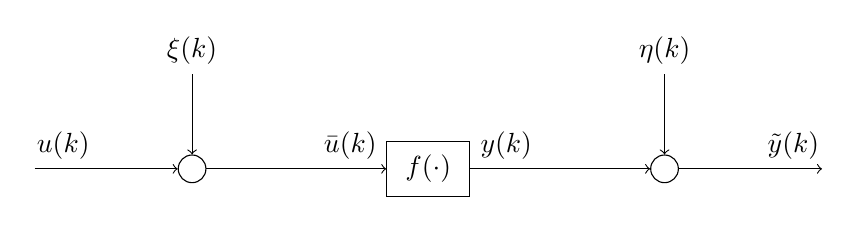
\begin{tikzpicture}[auto, node distance=2cm]

    % Block styles
    \tikzstyle{block} = [draw, rectangle, minimum height=2em, minimum width=3em]
    \tikzstyle{sum} = [draw, circle, inner sep=0pt, minimum size=1em]
    \tikzstyle{input} = [coordinate]
    \tikzstyle{output} = [coordinate]

    % Nodes
    \node [input] (input) {};
    \node [sum, right of=input, node distance=2cm] (sum1) {};
    \node [block, right of=sum1, node distance=3cm] (system) {$f(\cdot)$};
    \node [sum, right of=system, node distance=3cm] (sum2) {};
    \node [output, right of=sum2, node distance=2cm] (output) {};

    % Connections
    \draw [->] (input) -- node[pos=0.2] {$u(k)$} (sum1);
    \draw [->] (sum1) -- node[pos=0.8] {$\bar{u}(k)$} (system);
    \draw [->] (system) -- node[pos=0.2] {$y(k)$} (sum2);
    \draw [->] (sum2) -- node[pos=0.8] {$\tilde{y}(k)$} (output);
    
    % Noise terms
    \node [above of=sum1, node distance=1.5cm] (xi) {$\xi(k)$};
    \draw [->] (xi) -- (sum1);
    
    \node [above of=sum2, node distance=1.5cm] (eta) {$\eta(k)$};
    \draw [->] (eta) -- (sum2);

\end{tikzpicture}
\end{center}

\textit{Errors-in-variables} (EIV) problems refer to the most general case where both the input and the output collected samples are affected by noise.

\[
\xi = [\xi(1), \dots, \xi(H)] \in \mathcal{B}_{\xi}
\]
\[
\eta = [\eta(1), \dots, \eta(H)] \in \mathcal{B}_{\eta}
\]

$\mathcal{B}_{\xi}$ and $\mathcal{B}_{\eta}$ are bounded sets described by \textbf{\textit{polynomial constraints}.}

Most common case:
\[
\mathcal{B}_{\eta} = \left\{\eta : |\eta(k)| \leq \Delta_{\eta}\right\}, \quad \mathcal{B}_{\xi} = \left\{\xi : |\xi(k)| \leq \Delta_{\xi}\right\}
\]
which is a hyper-dimensional box.

A subset of this problem, as was discussed also in the previous chapter, is Output-Error, OE, set-up, meaning that the input signal is perfectly known.


\begin{center}    % Block styles
\begin{tikzpicture}[auto, node distance=2cm]

    \tikzstyle{block} = [draw, rectangle, minimum height=2em, minimum width=3em]
    \tikzstyle{sum} = [draw, circle, inner sep=0pt, minimum size=1em]
    \tikzstyle{input} = [coordinate]
    \tikzstyle{output} = [coordinate]

    % Nodes
    \node [input] (input) {};
    \node [block, right of=input, node distance=3cm] (system) {$f(\cdot)$};
    \node [sum, right of=system, node distance=3cm] (sum2) {};
    \node [output, right of=sum2, node distance=2cm] (output) {};

    % Connections
    \draw [->] (input) -- node[pos=0.5] {$u(k)$} (system);
    \draw [->] (system) -- node[pos=0.2] {$y(k)$} (sum2);
    \draw [->] (sum2) -- node[pos=0.8] {$\tilde{y}(k)$} (output);
    
    % Noise terms at the output
    \node [above of=sum2, node distance=1.5cm] (eta) {$\eta(k)$};
    \draw [->] (eta) -- (sum2);
\end{tikzpicture}
\end{center}\vspace{1cm}
where,
\begin{itemize}
\item 
\[
\eta = \left[\eta(1),\,\eta(2),\, \cdots,\,\eta(H)\right] \in \mathbb{B}_\eta
\]
\item \(\mathbb{B}_\eta\) is a bounded set described by \textbf{\textit{polynomial constraints}}.
\item Most common case: \(\mathbb{B}_\eta = \left\{\eta: \: |\eta(k)| \leq \Delta_\eta \right\}\)
\end{itemize}

The FPS for the general EIV problem is implicitly defined as follows:
\[
\begin{array}{c}
\mathbb{D}_\theta = \{ \theta \in \mathbb{R}^n : \, y(k) = f( y(k-1), y(k-2), \cdots, y(k-n),  u(k), u(k-1), \cdots \\[1ex]
, u(k-m), \theta_1, \theta_2, \cdots, \theta_{n+m+1}),k = n+1,\,n+2,\,\cdots,\,N,\: y(k) = \tilde{y}(k) - \eta(k), \\[1ex]
u(k) = \tilde{u}(k) - \xi(k),\: k=1,\,2,\,\cdots,\,N,\: |\xi(k)|\leq \Delta\xi(k),\: |\eta(k)\leq \Delta\eta(k),\: k = 1,\,2,\,\cdots,\,N \}
\end{array}
\]

The FPS for the case of \textbf{LTI descrete-time systems with EIV noise structure} is given by:
\[
\mathbb{D}_\theta = \left\{ \theta \in \mathbb{R}^p : \, (\tilde{y}(k) - \eta(k)) + \sum_{i=1}^{n} a_i (\tilde{y}(k - i) - \eta(k - i)) = \sum_{j=0}^{m} b_j (\tilde{u}(k - j) - \xi(k - j)), \right.
\]
\[
\left. t = n + 1, \dots, H, \quad |\xi(k)| \leq \Delta\xi(k), \quad |\eta(k)| \leq \Delta\eta(k), \quad k = 1, \dots, H \right\}
\]
This includes \(2N\) new variables involved in the FPS which are not variables in parameter space. Now, these variables should be eliminated, and this is not possible without setting some conservative conditions. \textbf{If you come up with an idea to do so without considering conservative conditions, you can publish a paper}. 

Since the FPS defined in the above equation depends on some additional unknownes( all the samples of the noise sequences). The constraints defining \(\mathbb{D}_\theta\) cannot be rearranged in such a way to eliminate dependancies on such additional variables. To solve the problem, we need to extend the space of decision variables in by defining the \textit{Extended Feasible Parameter Set}(EFPS).

\[
\begin{array}{c}
\mathcal{D}_{\theta,\eta,\xi} = \left\{ \theta \in \mathbb{R}^p, \eta \in \mathbb{R}^H, \xi \in \mathbb{R}^H : \right.
(y(k) - \eta(k) + \sum_{i=1}^{n} a_i ( y(k-i) - \eta(k-i)) = \\[2ex]
\sum_{j=0}^{m} b_j ( u(k-j) - \xi(k-j) ), \, t = n+1,\dots,H, \\[2ex]
|\xi(k)| \leq \Delta \xi(k), \, |\eta(k)| \leq \Delta \eta(k), \, k = 1,\dots,H \left.\right\}
\end{array}
\]
As you can see in the box below, here, we are expanding the space we are considering for FPS, hence EFPS.
\begin{align}
\fcolorbox{red}{white}{$\mathcal{D}_{\theta,\eta,\xi} = \left\{ \theta \in \mathbb{R}^p, \eta \in \mathbb{R}^H, \xi \in \mathbb{R}^H\right\}$}
\end{align}

A simplified graphical varsion is going to be like the following graph:

\begin{figure}[htbp]  % "h" for here, "t" for top, "b" for bottom, "p" for float page
    \centering
    \includegraphics[width=0.7\textwidth]{images/EFPS.png}
    \caption{A simplified, general graph of EFPS.}
    \label{fig:EFPS}
\end{figure}

In this case,
\[
\underline{\theta}_k = \min\limits_{\theta \in \mathbb{D}_\theta} \theta_k = \min\limits_{\theta, \eta, \xi \in \mathbb{D}_{\theta, \eta, \xi}} \theta_k
\]
That is,
\[
\begin{array}{rcl}
\theta_k & = & \min_{\theta \in \mathbb{D}_\theta, \eta, \xi} \theta_k \text{ subject to } \tilde{y}(k) - \eta(k) + \sum_{i=1}^{n} \theta_i(\tilde{y}(k-i) - \eta(k-i)) \\[1ex]
& = & \theta_{n+1}(\tilde{u}(k) - \xi(k)) + \sum_{j=1}^{m} \theta_{n+j+1}(\tilde{y}(k-j) - \xi(k-j)), \\[1ex]
& & \quad \forall k > n+1, \, |\xi(k)| \leq \Delta \xi, \, |\eta(k)| \leq \Delta \eta, \, \forall k
\end{array}
\]

The drawback is that EFPS is a non-convex set defined by \textbf{polynomial} (\textit{bilinear}) constraints.

\begin{factbox}[Professor's Quote:]
To the best of my knowledge, in the domain of non-convex functions, the only class that can be optimized up to the global minimum is the class of non-convex functions with polynomial constraints.
\end{factbox}


\chapter{Continuous-time identification}
We start this discussion considering LTI SISO models.



\chapter{Laboratory 01: solution}

Upon successful completion of this homework, students will
\begin{enumerate}
\item Be able to compute Least Squares (`2 norm) and Least `∞ norm parameter estimation for
Discrete-time LTI systems.
\item Be able to analyze properties and limitations of the considered estimators
\end{enumerate}

The plant to be estimated is a continuous-time LTI dynamical system assumed to be exactly described by the following transfer function:
\[
G_p(s) = \frac {100}{s^2 + 1.2 s + 1}
\]

Assuming the sampling time \(T_s = 1\), the following script is used for discretizing the transfer function of the sysetm, using \textit{zoh}, or zero-order-hold method.

\[G_d = c2d(G_p, Ts, 'zoh')\]

The result going to be of the following form:

\[G_d(z) = \frac{N(z)}{D(z)}\]

The result of this command is as follows:

\[
G_d(z) = \frac{32.24z + 21.41}{z^2 - 0.7647z + 0.3012}
\]

Now, the input of the system is considered to be samples of a uniformly distributed random variable. The command \textit{\(u = rand(N,1)\)} is used at this end. \(N\) is considered to be 1000. Then, the command \textit{ \(y =\)lsim(\(G_d, u, Ts)\)} is used to simulate \textbf{noise-free} output samples. Here, it is assumed that the input of the system is exactly known.


\subsubsection{\(\theta_{LS}\) in ideal noise-free setting}
The regression matrix \(A\) and output vector \(b\), are shaped as follows. It is worthwhile to mention that, in this case, since the samples are noise free, \(N = 7\) suffice to obtain exactly the the values of the parameters.

\[
    y_{Noise Free} = A_{Noise Free}\theta
\]
where \(y = [y(3) y(4) ... y(N)]^T, \theta = [\theta_1 \theta_2 ... \theta_5]^T)\), and
\[
    A = \left[
    \begin{matrix}
    -y(2) & -y(3) & u(3) & u(2) & u(1) \\
    -y(3) & -y(2) & u(4) & u(3) & u(2) \\
    \cdots & \cdots & \cdots & \cdots & \cdots   \\
    \cdots & \cdots & \cdots & \cdots & \cdots   \\
    -y(N-1) & -y(N-2) & u(N) & u(N-1) & u(N-2)
    \end{matrix} 
    \right]\\
\]
The command used for deriving \(\theta's\) is:
\[
\theta_{LS} = y \ A
\]

It can be seen that the parameters obtained in this way are exactly parameters of the discretized transferfunction, except for arithmatic roundings.
\[
\begin{bmatrix}
    \theta_{LS} & \theta_{Gd} \\
    -0.7647 & -0.7647 \\
     0.3012 & 0.3012 \\
    -0.0000 & 0 \\
    32.2369 & 32.2369 \\
    21.4103 & 21.4103
\end{bmatrix}
\]

\subsubsection{\(\theta_{LS}\) in Equation-Error setting}
In the second part, it is asked to repeat the process of estimation, simulating an error that affect the equation. In this case the collected measurement y are give by:
\[
D_d(q^{-1})y_t = N_d(q^{-1})u_t + e_t
\]
\begin{QandAbox}
This assumption about the noise structure is theoretical, and it is not according to read data acquisition setting, which is Error-in-Variable setting or, assuming input to be exactly known Output-Error setting
\end{QandAbox}
Here, the error, \(e\), is considered to be a normaly distributed noise with standard deviation 5.
\[
e = 5 * randn(N,1)
\]

To create output data samples that is affected in this manner, the noise entering each output sample should be filtered by \(D(z)\)the denuminator of \(G_d\). Therefore the following MATLAB code should be used:
\[
\text{[num, den]} = tfdata(Gd, 'v')
y\_EE = lsim(Gd,u) + lsim(tf(1,den),e)
\]

In this case, the regression matrix is shaped by the noisy output samples. Hence:
\(y_{EE} = [y_{EE}(3) \: y_{EE}(4) ... y_{EE}(N)]^T 
\)
\[
    A = \left[
    \begin{matrix}
    -y_{EE}(2) & -y_{EE}(3) & u(3) & u(2) & u(1) \\
    -y_{EE}(3) & -y_{EE}(2) & u(4) & u(3) & u(2) \\
    \cdots & \cdots & \cdots & \cdots & \cdots   \\
    \cdots & \cdots & \cdots & \cdots & \cdots   \\
    -y_{EE}(N-1) & -y_{EE}(N-2) & u(N) & u(N-1) & u(N-2)
    \end{matrix} 
    \right]\\
\]

The result of the Least square algorithm is going to be as follow:
\[
\begin{bmatrix}
    \theta_{EE} & \theta_{Gd} \\
    -0.7762 & -0.7647 \\
     0.3116 & 0.3012 \\
     0.2078 & 0 \\
    32.2405 & 32.2369 \\
    21.0843 & 21.4103
\end{bmatrix}
\]
As it can be seen, the result is very close to the observed values. Since this structure of the noise satisfies both assumptions of the consistency property of Least Squares, it is guaranteed that as \(N\) tends to infinity, the values of \(\theta\) will converge to the true values, regardless of how large the standard deviation of the noise affecting

\subsubsection{\(\theta_{LS}\) in Output-Error setting}
The noise in this setting directly affect the output measurements
\[
y_t = G_d(q^{-1})u_t + \eta_t
\]
\begin{QandAbox}
This setting is a good structure compliant with the real data acquisition setting.
\end{QandAbox}
Here, the error, \(\eta_t\), is considered to be a normaly distributed noise with standard deviation 5.
\[
eta = 5 * randn(N,1)
\]

To create output data samples that is affected in this manner, the following MATLAB code should be used:
\[
y\_OE = lsim(Gd,u) + eta
\]

In this case, the regression matrix is shaped by the noisy output samples. Hence:
\(y_{OE} = [y_{OE}(3) \: y_{OE}(4) ... y_{OE}(N)]^T 
\)
\[
    A = \left[
    \begin{matrix}
    -y_{OE}(2) & -y_{OE}(3) & u(3) & u(2) & u(1) \\
    -y_{OE}(3) & -y_{OE}(2) & u(4) & u(3) & u(2) \\
    \cdots & \cdots & \cdots & \cdots & \cdots   \\
    \cdots & \cdots & \cdots & \cdots & \cdots   \\
    -y_{OE}(N-1) & -y_{OE}(N-2) & u(N) & u(N-1) & u(N-2)
    \end{matrix} 
    \right]\\
\]

The result of the Least square algorithm is going to be as follow:
\[
\begin{bmatrix}
    \theta_{OE} & \theta_{Gd} \\
    -0.5369 & -0.7647 \\
     0.1352 & 0.3012 \\
    -0.2887 & 0 \\
    32.0653 & 32.2369 \\
    28.1921 & 21.4103
\end{bmatrix}
\]
Since this noise structure does not satisfy the second assumption of the consistency property of the least square method, no matter how large \(N\) is, the estimation values are not going to converge to the real values.

DO THE LAB 1 WITH NORM INF

\chapter{Laboratory 02: solution}

In this problem we assume that the plant to be identified is exactly described as a discrete-time
LTI models described by the following transfer function (in the \(q^{-1}\) operator):
\[
G_p(q^{-1}) = \frac {\theta_2}{1 + \theta_1q^{-1}}
\]
where
\[
\theta = \left[-0.5 2 \right]
\]
Now, it is required to compute a set-membership estimation of the parameters of the system by means of the following procedure:\\
Assume that the uncertainty affecting the input output data enters the problem according to an equation error structure. Furthermore, to perform the simulation, assume that collected input sequence \(\tilde{u}\) and the unknwon equation error sequences e are as follows :
\[
\tilde{u} = \left[4,\,-3,\,2,\, 1 \right]^T
\]
and
\[
e = \left[0.05,\,-0.25,\,0.3,\,-0.5 \right]^T
\]
Perform a simulation of model in order to collect the input and output data to be used for identification. The output sequence \(tilde{y}\) has to be computed according to the following equation (equation error structure):\\
Based on the transfer function at hand the difference equation of the system is as follow:
\[
y(k) = -\theta_1y(k-1) + \theta_2u(k)
\]
Considering an \textit{Equation-Error} structure for the noise, the following relationship is obtained:
\[
\tilde{y}(k) = -\theta_1 \tilde{y}(k-1) + \theta_2u(k) + e(k)
\]
Where it is assumed that the error \(e\) is known to be bounded as \(|e(k)|\leq \Delta e\) and assuming as initial condition \(\tilde{y}\).

Considering the difference equation of the system, the following information can be obtained:\\
\begin{itemize}
\item \(n_a = 1\) which represent the order of the system, which corresponds to the number of previous samples of \(y\) needed to express the difference equation of the system.
\item \(n_b\) the number of input samples in the difference equation.
\item \(t_{min} = \max(\left[n_a +1, n_b\right]\)
\end{itemize}
MATLAB code for simulation of the system is as follows:

\begin{example}
\begin{lstlisting}[caption=Set-membership estimation with theta bounds and simulation]
close all
clear variables
clc
format compact

%% Defining system
z = tf('z',1);
theta = [-0.5 2];
Gp = theta(2)/(1 + theta(1)*z)

u_tilde = [4 -3 2 1]';
e = [0.05 -0.25 0.3 -0.5]';

%% Simulation
% y_tilde(k) = -theta_1*y_tilde(k-1) + theta_2 u_tilde(k) + e(k)
na = 1; % The number of state variables or last samples of y
nb = 1; % The number of past inputs
N = 4;
t_min = max([na+1 , nb]);
y_tilde = zeros(4,1); 
% Initial value

for k = t_min:N
    y_tilde(k) = -theta(1)*y_tilde(k-1) + theta(2)*u_tilde(k) + e(k);
end

%% Upper and lower bound
delta_e = 0.5;
y_up = y_tilde + delta_e;
y_low = y_tilde - delta_e;
plot(1:N, [y_up, y_tilde, y_low])
\end{lstlisting}
\end{example}

In order to obtain \textit{Feasible Uncertainty Set}, it is required to do the following manipulations, considering the definition of FPS we have:
\[
\mathbb{D}_\theta = \left\{ \theta | \tilde{y}(k) + \theta_1 \tilde{y}(k-1) + \theta_2\tilde{u}(k)| \leq \Delta e \forall k \right\}  
\]
Writing exampding the equations for \(t_{min}\) to \(N = 4\), which is the number of samples, we obtain:
\begin{align*}
|\tilde{y}(2) + \theta_1 \tilde{y}(1) + \theta_2\tilde{u}(2)| &\leq \Delta e \\
|\tilde{y}(3) + \theta_1 \tilde{y}(2) + \theta_2\tilde{u}(3)| &\leq \Delta e \\
|\tilde{y}(4) + \theta_1 \tilde{y}(3) + \theta_2\tilde{u}(4)| &\leq \Delta e
\end{align*}
and therefore,
\begin{align*}
-\Delta e - \tilde{y}(2) \geq \theta_1 \tilde{y}(1) + \theta_2\tilde{u}(2) &\leq \Delta e - \tilde{y}(2) \\
-\Delta e - \tilde{y}(3) \geq \theta_1 \tilde{y}(2) + \theta_2\tilde{u}(3) &\leq \Delta e - \tilde{y}(3) \\-\Delta e - \tilde{y}(4) \geq \theta_1 \tilde{y}(3) + \theta_2\tilde{u}(4) &\leq \Delta e - \tilde{y}(4) 
\end{align*}

In each of these relationships, each inequality is a constraint in parameter space that needs to be satisfied so that the equation error becomes less that \(\Delta e\). For finding \(\mathbb{D}_\theta\) in the parameter space, we can consider inequalities as equality, and by doing so, we obtain the equation of 3 pairs of parallel lines on the parameter space, which in this case is a two-dimensional plane. After writing the following MATLAB code, the intersections of all the regiones between the top bound and lower bounds lead to FPS. The plot of the feasible uncertaintly set in the parameter space is as follows:
\begin{example}
\begin{lstlisting}
%% Theta_1 variation
theta_1 = linspace(-5, 5, 1000);
figure,
hold on
for k = t_min:N
    theta_2_up = (+delta_e + y_tilde(k) + theta_1*y_tilde(k-1)) / u_tilde(k);
    theta_2_low = (-delta_e + y_tilde(k) + theta_1*y_tilde(k-1)) / u_tilde(k);
    plot(theta_1, theta_2_low, 'b')
    plot(theta_1, theta_2_up, 'r')
end

%% Brute-force approach (not recommended)
figure,
hold on
for theta_1 = -100:0.01:100
    for theta_2 = -100:0.01:100
        for k = t_min:N
            f = 1; % Flag
            if(abs(y_tilde(k) + theta_1*y_tilde(k-1) - theta_2*u_tilde(k)) > delta_e)
                f = 0;
                break
            end
        end
        if (f == 1)
            plot(theta_1, theta_2, '+');
        end
    end
end
\end{lstlisting}
\end{example}


\begin{figure}[htbp]  % "h" for here, "t" for top, "b" for bottom, "p" for float page
    \centering
    \includegraphics[width=0.65\textwidth]{images/FPS.jpg}
    \caption{FPS represented in the parameter space; the horizontal axis is \(\theta_1\) and the vertical axis is \(\theta_2 \)}
    \label{fig:PFS}
\end{figure}

It can be seen that the "real value" of the parameters is one of point at the top left corner of the \(\mathbb{D}_\theta\).


\chapter{Laboratory 02b: solution}
\begin{QandAbox}
In order to solve this problem, \textit{SparsePOP} and \textit{Sedumi}, toolboxes should be installed, there exist one tutorial file.
\end{QandAbox}
consider the following problem:
\[
\begin{array}{c}
x^* = \arg\,\min\limits_{x} x_1^2 + x_2^2 - 4x_1 - 6x_2 + 13\\
\text{ s.t. }\\[1em]
x_1x_2 - 7x_2 = 10\\ [1em]
x_2 \geq -\frac{1}{2}x_1 +1
\end{array}
\]
The cost function here is a polynomial, which is a sum of \textit{monomial} terms. Each monomial is of the following form:
\[
\alpha x_1^{C_1} x_2^{C_2} \cdots x_n^{C_n}
\]

\begin{example}[Drawing the contour]
\begin{lstlisting}
clear; close all; clc;

%% Part 1: plot
x1_lw = -15; x1_up = +15;
x2_lw = -12; x2_up = +12;

x1 = linspace(x1_lw, x1_up);
x2 = linspace(x2_lw, x2_up);
% objective function
[X1,X2] = meshgrid(x1,x2);
Z = X1.^2 + X2.^2 - 4.*X1 - 6.*X2 + 13;
figure, contour(X1,X2,Z,5*(1:50)');

% equality constraint
x2_1 = linspace(0.01, x2_up);
x2_2 = linspace(x2_lw, -0.01);
x1_1 = (10+7.*x2_1)./x2_1;
x1_2 = (10+7.*x2_2)./x2_2;
hold on; plot(x1_1,x2_1, 'k',x1_2,x2_2, 'k');
axis([x1_lw,x1_up,x2_lw,x2_up]);
\end{lstlisting}
\end{example}


\begin{example}
\begin{lstlisting}
% inequality constraint
x2_ineq = -0.5*x1 + 1;
hold on; plot(x1, x2_ineq, 'b');
patch([x1(1); x1(end); x1_up; x1_lw], ...
    [x2_ineq(1); x2_ineq(end); x2_up; x2_up], ...
    'blue', 'FaceColor', 'blue', 'FaceAlpha', 0.1);
\end{lstlisting}
\end{example}
The resultant graph is as follows:

\begin{figure}[htbp]  % "h" for here, "t" for top, "b" for bottom, "p" for float page
    \centering
    \includegraphics[width=0.75\textwidth]{images/lab02_contour.jpg}
    \caption{The contour of the polynomial as well as the graph of the constraints}
    \label{fig:constraints}
\end{figure}

Let's create the polynomial to be minized, named \textbf{objPoly}:

\begin{example}[Definig the polynomila to be optimized]
\begin{lstlisting}
% objective function
objPoly.noTerms = 5;
objPoly.dimVar = 2;
objPoly.typeCone = 1;  %always to be set to 1
objPoly.degree = 2; %the degree of the poly
objPoly.supports = [2 0; 0 2; 1 0; 0 1; 0 0];
objPoly.coef = [1, 1, -4, -6, 13]'; %should be a column vector
\end{lstlisting}
\end{example}
Pay attention that the support matrix should be made according to the following scheme:

\begin{figure}[ht]  % "h" for here, "t" for top, "b" for bottom, "p" for float page
    \centering
    \includegraphics[width=0.75\textwidth]{images/support-matrix.png}
    \caption{The contour of the polynomial as well as the graph of the constraints}
    \label{fig:constraints}
\end{figure}

The inequality and equality constraints should be defined as cell array structures. Pay attention that:
\begin{itemize}
\item \textbf{Equality}: .typeCone = -1
\item \textbf{Inequality}: .typeCone = 1
\end{itemize}

\begin{example}[Definig the polynomila to be optimized]
\begin{lstlisting}
% equality constraint
c = 1;
ineqPolySys{c}.noTerms = 3;
ineqPolySys{c}.dimVar = 2;
ineqPolySys{c}.typeCone = -1; % equality
ineqPolySys{c}.degree = 2;
ineqPolySys{c}.supports = [1 1; 0 1; 0 0];
ineqPolySys{c}.coef = [1 -7 -10]';
% inequality constraint
c = 2;
ineqPolySys{c}.noTerms = 3;
ineqPolySys{c}.dimVar = 2;
ineqPolySys{c}.typeCone = +1; % inequality
ineqPolySys{c}.degree = 1;
ineqPolySys{c}.supports = [0 1; 1 0; 0 0];
ineqPolySys{c}.coef = [1 0.5 -1]';
\end{lstlisting}
\end{example}

After defining the lower bounds and upper bounds for the optimization variables, the \textbf{relaxation order} should be chosen. For this lab, it is recommended that one tries with relaxation orders 1, 2, 3, 4 to solve the problem.

\begin{example}[Solving the optimization problem]
\begin{lstlisting}
% lower bound
lbd = -1e10*ones(2,1);
% upper bound
ubd = +1e10*ones(2,1);

param.relaxOrder = 3;
param.POPsolver = 'interior-point';

[a,b,POP] = sparsePOP(objPoly, ineqPolySys, lbd, ubd, param);
sol_relaxed = POP.xVect;
sol_refined = POP.xVectL;

hold on; 
plot(sol_relaxed(1),sol_relaxed(2),'r*');
plot(sol_refined(1),sol_refined(2),'m*');
\end{lstlisting}
\end{example}

For relaxation order 1 and 2, it can be seen that the solution of the optimization problem does not respect the constraints. That is, the solution is not acceptable.

\begin{figure}[htbp]  % "h" for here, "t" for top, "b" for bottom, "p" for float page
    \centering
    \includegraphics[width=0.75\textwidth]{images/relaxed1.jpg}
    \caption{The solution of the problem with relaxation order 1, the red star spots the relaxed solution and the other star the refined solution, which is the result of sedumi}
    \label{fig:constraints}
\end{figure}

With the relaxation order 3, the problem has an acceptable solution.


\begin{figure}[htbp]  % "h" for here, "t" for top, "b" for bottom, "p" for float page
    \centering
    \includegraphics[width=0.75\textwidth]{images/relax3.jpg}
    \caption{The solution of the problem with relaxation order 3}
    \label{fig:constraints}
\end{figure}

\chapter{Laboratory 04: solution}
In this problem we assume that the plant to be identified is exactly described as a discrete-time
LTI models described by the following transfer function:
\[
G_p(q^{-1}) = \frac{N(q^{-1})}{D(q^{-1})} = \frac{\theta_3 + \theta_4 q^{-1} + \theta_5 q^{-2}}{1 + \theta_1 q^{-1} + \theta_2 q^{-2}} 
\]
\subsubsection{Data acquisition considerations:}
\begin{itemize}
    \item \textbf{Sampling rate: }As a rule of thumb, we should have at least 20 to 50 data from the transient of the system. Therefore, first, we apply a step to the system and we see the setteling time of the system, if this value is devided by 50 we obtain the period of the sampling. For this lab, setteling time is around 0.5, so the sampling rate should be at least 100. It was recommended to perform the lab with the sample rate around 250. \\
    It was also recommended to acquisit data with higher sampling rates such as 500 and 1000. It was suggested that we are going to face an issue regarding theoretical aspects of control thoery, yet to be explained. (I guess that maybe it makes the identification more dependent on the noise since we are introducing more noise to the data).
    \item \textbf{Bounds on the noise:} In order to have an idea about the bound of the noise, it was recommended to acquisit data with zero input, or at any rate without any input, and then, have an idea about the input and output noise bounds.
    \item \textbf{Input signal} It was recommended to use \textbf{uniformly distributed random signal}, but care should be taken regarding the amplitude of the noise. \begin{itemize}
                \item \textbf{too low amplitude} $\Rightarrow$ \textbf{bad SNR}, Signal to Noise Ratio.
                \item \textbf{too high amplitude} $\Rightarrow$ \textbf{Risk of saturation}, having non-linearity which is not assumed.\\
                \end{itemize}
                
                Considering the inputs with \textbf{DC gains}, so that you excite better the low-frequency range of frequency spectrum. Not too much! since a large DC and large amplitude may lead to saturation of the output. 
     
    \item In the lab assignment, it is required to stimulate the system with a square wave input, and acquire samples for identification purposes.
\end{itemize}


% ---------------------------------------------------------------------
% ---------------------------------------------------------------------
% ---------------------------------------------------------------------

% Declare appendix and set the equation counter format to (A.section.eqNumber)
\appendix
\renewcommand{\theequation}{\thesection.\arabic{equation}}
\input{chapters/Appendix}

\end{document}
